%11.   State of the Art (or Related Work or Literature Review)
%In this section you should present the theoretical basis of your work and overview of the existing solutions. When discussing on the exiting solutions you should relate and qualitatively compare them with yours. This chapter should contain:

% 1) The theory and concepts of your work. For example, if you work on compiler you can mention about how compiler works without getting much into detail.

% 2) Existing state of the art solution. For example, if you implement an optimization pass, you should mention about existing optimization passes that are relevant with yours. You should emphasize the commons and differences with your solution and with the existing ones.

% You may divide this chapter in sections (e.g. each for the different existing solution).

\section{Overview}
\label{sec:overview} 

\subsection{Preliminaries}
\label{sec:theory} 

% The theory and concepts of your work. For example, if you work on compiler you can mention about how compiler works without getting much into detail.

\newcommand{\argmin}{\operatornamewithlimits{arg\,min}}
\newcommand{\Bx}{{\bf x}}
\newcommand{\By}{{\bf y}}
\newcommand{\Bh}{{\bf h}}
\newcommand{\Bw}{{\bf w}}
\newcommand{\Bc}{{\bf c}}

In this section we will describe the basics of artificial neural networks. We will also introduce the notation used in this work. Note that the definitions and notations vary through the literature. We use the one which the author is familiar with. For the reader who is comfortable with this topic we recommend to skip this section and go to related models \ref{sec:overview-models}. 

TODO notation about datasets as input / output vector, sample, sample set, training, test + citation. Stopping criterion. 

%=============================================================
\subsubsection{Perceptron.}
\label{sec:models-perceptron}

The theory behind artificial neural networks started with the model of \emph{Perceptron} introduced by~\citet{mcculloch1943logical}. It is a simple model which transforms a vector of inputs $s$ to an output value $y$. The notation as depicted on figure~\ref{fig:perceptron}: $x$ is the \emph{input vector} where always $x_0=1$, $w_{0k}$ is the \emph{weight} vector, $\Sigma$ is the \emph{summing} junction, $\eta_k$ is the \emph{net input}, $\phi$ is the \emph{activation function}, $\theta_k$ is the \emph{treshold}, $y_k$ is the \emph{output} and $b_k$ is the \emph{bias}.

\begin{figure}[H]
  \centering
  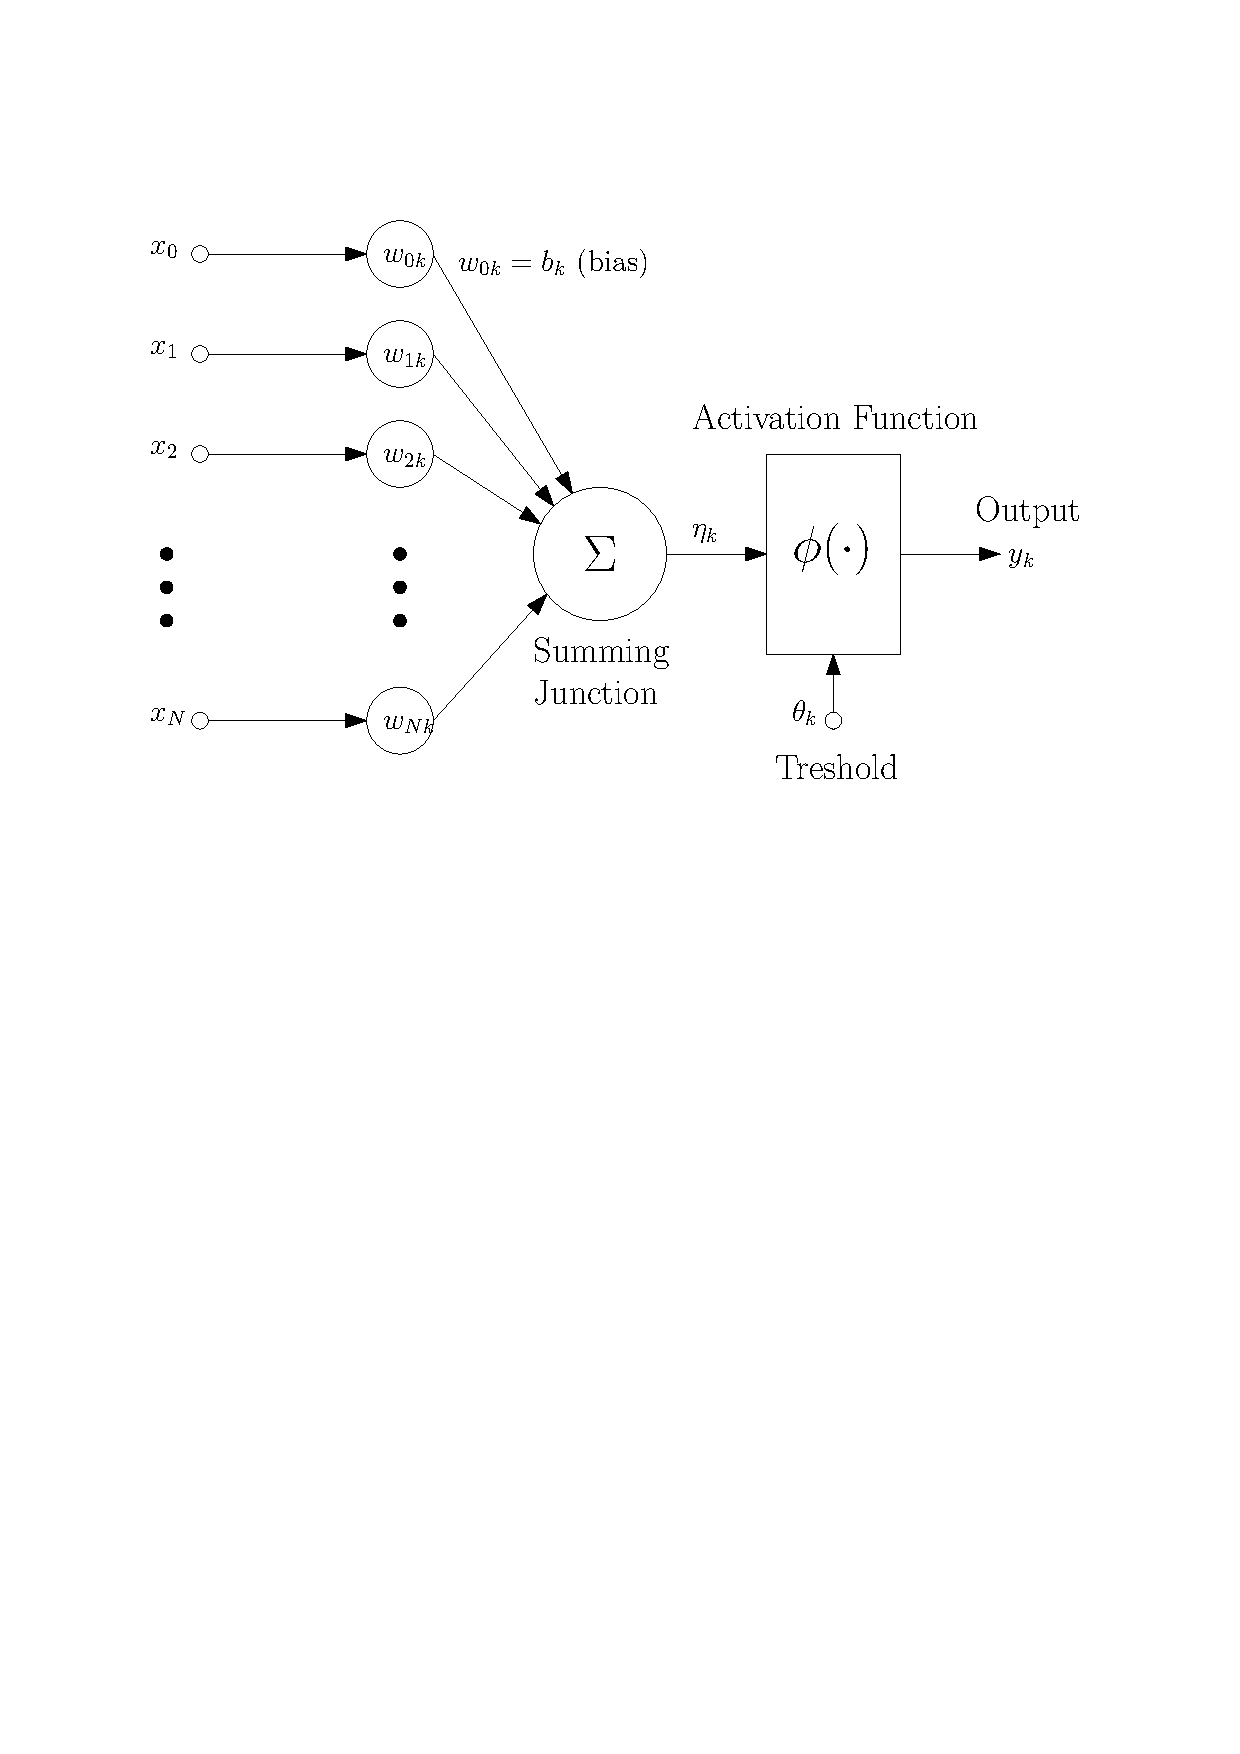
\includegraphics[width=0.6\textwidth]{img/perceptron.pdf}    
  \caption{Perceptron transforming \emph{inputs} $[x_0,\, x_1,\, \ldots,\, x_N]$ to \emph{output} $y_k$.} 
  \label{fig:perceptron}
\end{figure}

The whole transformation of the input vector to the output activation could be written as follows: 
\begin{equation}
\label{eq:perceptron} 
y_k =
\left\{
	\begin{array}{ll}
		1 & \mbox{if } \phi(\sum_{i=0}^N x_iw_{ik}) > \theta_k \\
		0 & \mbox{otherwise}
	\end{array}
\right.
\end{equation} 

Equation~\ref{eq:perceptron} describes a simple \emph{binary treshold perceptron}. One could observe that the binary perceptron divides the vector space $\mathbb{R}^N$ by a $(n-1)$--dimensional hyperplane. This behaviour was studied by~\citet{rosenblatt1958perceptron}. Now we see the importance of bias which is the absolute term in the equation of the hyperplane. \label{sec:linear-sep} This leads to the fact that for one perceptron is impossible to classify non--\emph{linearly separable} vectors. 

\paragraph{Continuous perceptron.}
We put additional constraints for the activation function $\phi : \mathbb{R} \mapsto (0,1)$ that $\phi$ is differentiable, monotonously increasing and satisfying two asymptotic conditions $t(-\infty)=0$ and $t(\infty)=1$.  Usually, the activation function is realized by the logistic function $\frac{1}{1 + \exp{-\eta}}$. To allow real numbered results from the range $(0,1)$, we drop the treshold function and simply output $\phi(\eta_k)$. 

\paragraph{Learning.} 
The goal of a perceptron is to \emph{learn} the mapping given by the set $T = \{(X^j, t_j)\}$ of pairs, where $X^j$ is the input vector $(x_{j0},x_{j1}, \ldots, x_{jN})$ and $t_j$ is the corresponding target. It could be formalized as minimizing the error function: 

\begin{equation}
\label{eq:perceptron-error} 
E = \sum_{k=1}^{N} \frac{1}{2}(t_k-y_k)^2.
\end{equation} 

A straightforward method for the network to minimize the error function \ref{eq:perceptron-error} is simply updating weights according to the partial derivates of the error function: 

\begin{equation}
\label{eq:perceptron-learning} 
\frac{\partial E}{\partial w_{ik}} = (t_k - y_k)\phi'(\eta_k)x_i = (y_k - t_k)y_k(1 - y_k)x_i,
\end{equation} 
which gives us the \emph{update rule} written as: 
\
\begin{equation} 
\label{eq:perceptron-learning-rule} 
\Delta w_{ik} = \lambda (t_k - y_k)y_k(1 - y_k)x_i,
\end{equation} 
where $\lambda$ is the \emph{learning rate}. 

Using the learning rule~(\ref{eq:perceptron-learning-rule}) and the following \emph{training} process the perceptron is able to \emph{learn}: 
%TODO check algorithm 
\begin{algorithm}[H]
  \begin{algorithmic}
    \For{$epoch = 1$ to $Epoch_{\rm max}$} 
      \ForAll{$(X^j, t_j)$ in $T$} 
        \State $y_j \gets \phi(\sum_{i=0}^N x_iw_{ik}) > \theta_k$
        \For{$i=0$ to $N$} 
          \State $w_{ij} \gets w_{ij} + \lambda (t_k - y_k)y_k(1 - y_k)x_i$
        \EndFor
      \EndFor
    \EndFor
  \end{algorithmic}
  \caption{Perceptron learning. Applying the \emph{weight update rule}~\ref{eq:perceptron-learning-rule} in loop for each sample in $T$. One main loop is called \emph{epoch}.}  
  \label{alg:perceptron-learning}
\end{algorithm} 

 
\label{sec:perceptron} 

\subsubsection{Multilayer Feedworward Networks} 
\label{sec:theory-multilayer} 

We will define \emph{multilayer feedforward networks} as in \citet{haykin1994neural}. First, we define a \emph{layered} neural network where neurons are organised to form layers. In the simplest version we have an \emph{input layer} of source nodes and an \emph{output layer} which is formed by aforementioned perceptrons. In other words this is a \emph{feedforward} or \emph{acyclic} type of network as the \emph{activation}, i.e. outputs of the neurons are computed from the input to the output layer and never \emph{backwards}. 

Multilayer neural network has one or more \emph{hidden layers} in addition to the input and ouput layer as shown on figure~\ref{fig:multilayer}. The source nodes supply the activation pattern, i.e. input vector, which is applied to second layer neurons. The output signal of the hidden layer is used as the input for the output layer. As shown by \citet{cybenko1989approximation} the three layer network is an universal approximator continuous functions on compact subsets of $\mathbb{R}^n$.

\begin{figure}[H]
  \centering
  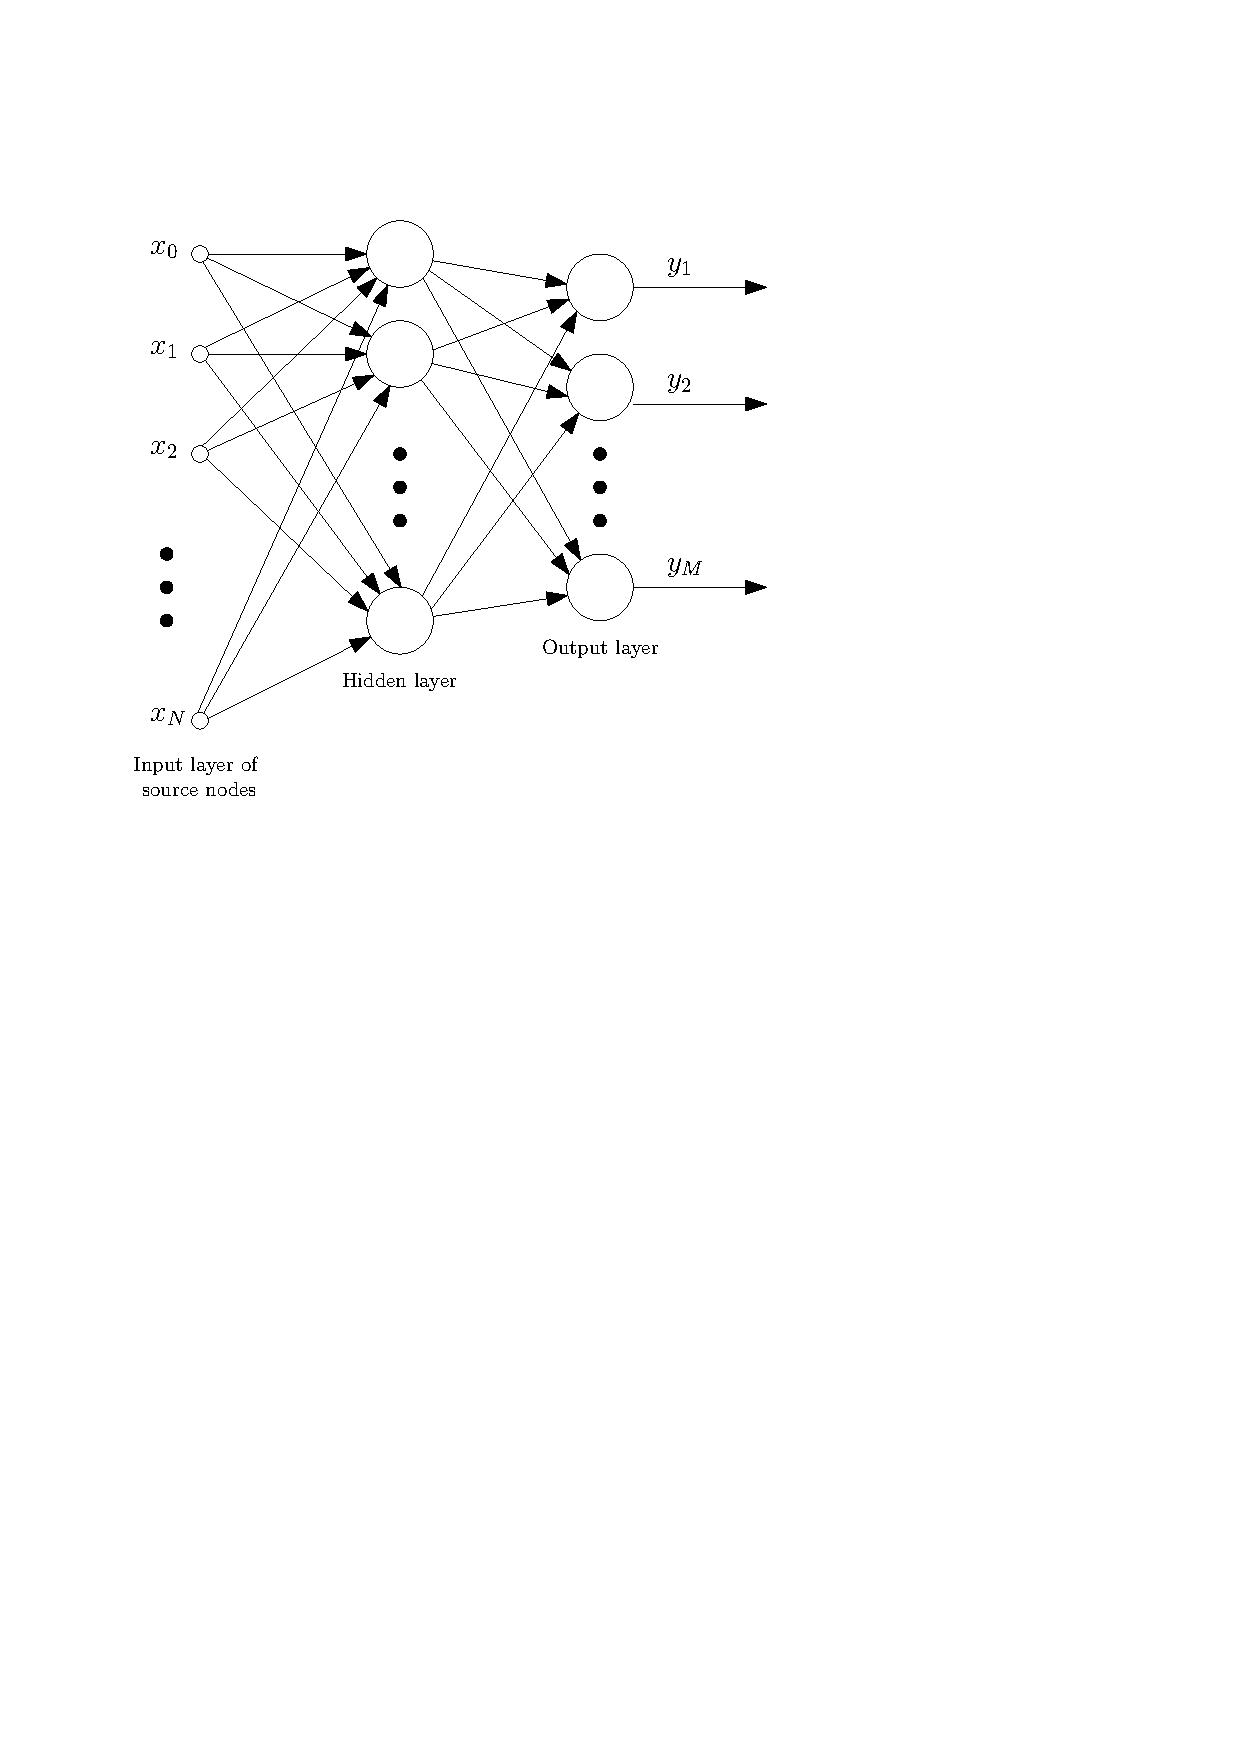
\includegraphics[width=0.5\textwidth]{img/multilayer.pdf}    
  \caption{Fully connected feedforward \emph{multilayer} network with one \emph{hidden} layer and one \emph{output} layer. } 
  \label{fig:multilayer}
\end{figure}

There exists several methods for training multilayer networks. First, we will describe the most common Backpropagation in (\ref{sec:models-bp}) and then methods related to our work such as CHL (\ref{sec:models-chl}), GeneRec (\ref{sec:models-generec}) and BAL (\ref{sec:models-bal}). 


\subsubsection{Recurrent Networks}
\label{sec:theory-recurrent} 

Recurrent networks arise problems with computing their activations. For example imagine a cycle of neurons. That means that output of a particular unit could affect its input. Therefore the activations in general couldn't be computed only by one forward pass. This introduces real--valued dynamic systems for computing the activations. We can observe that it holds that $\frac{\partial\eta}{\partial t} = 0$ for the activations of neurons in the fixed point state. There are several approaches solving these dynamic systems and deriving the learning rule \cite{pineda1987generalization, pearlmutter1989learning, williams1989learning, elman1990finding, haykin1994neural}. 

\begin{figure}[H]
  \centering
  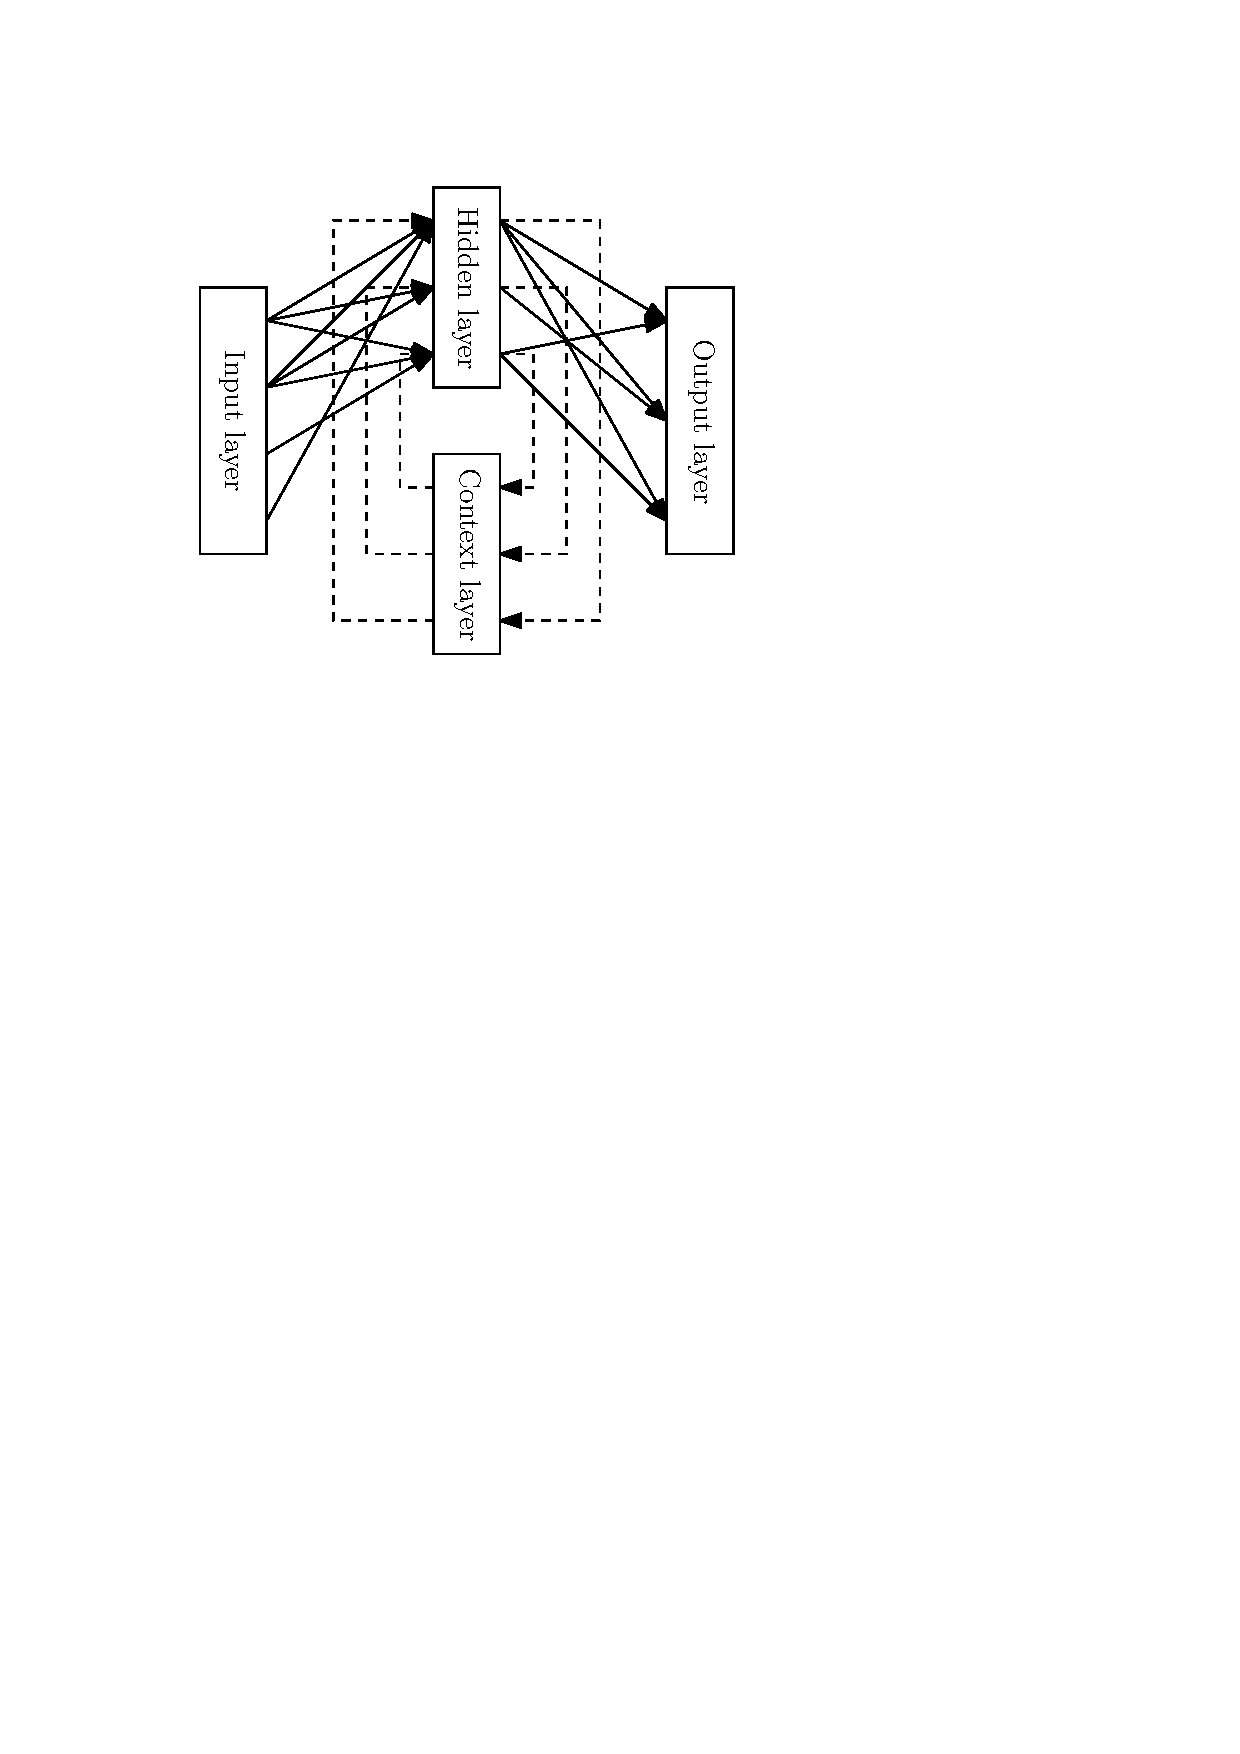
\includegraphics[width=0.4\textwidth]{img/models-recurrent.pdf}    
  \caption{Simple Recurrent network designed by \citet{elman1990finding}. Image inspiration from \citet{haykin1994neural}.} 
  \label{fig:theory-recurrent}
\end{figure}

An \emph{iterative method} is used by \citet{movellan1990contrastive} for computing activations. In the first step the input neurons have activations equal to the input vector and the other neurons have zero activation. In the next steps activations from the last step are used to compute activation in this step as shown in equation~\ref{eq:theory-recurrent-activation}: 
\begin{equation}
  \label{eq:theory-recurrent-activation} 
  \eta_i(t+1) = \phi(\sum_j w_{ji}\eta_i(t)
\end{equation}
This rule is iterated while the activation are settled. For particullar symmetric network it could be proved that activations will converge \citep{o1996bio}. For more general networks a dynamic system based on rule~\ref{eq:theory-recurrent-activation} could be derived and a fixed point solution could be found by solving a set of non--linear equations (TODO ref). \citet{movellan1990contrastive} proposes using the method of simulated annealing \citep{kirkpatrick1983optimization,vcerny1985thermodynamical} to improve the learning rule and to avoid settling the network in a local minima. We experimented with the iterative method for a two--way GeneRec \ref{sec:our-bal-recirc}. 

 

\subsubsection{Hopfield Networks}
\label{sec:theory-hopfield}

A \emph{Hopfield network} \citep{hopfield1984neurons} is a network with arbitrary connections defined only by one weight matrix $W$. Some of the units are chosen as the \emph{input units} which have stable activations for a given input pattern. We can treat a Hopfield network as a Recurrent neural network. A Hopfield network comes with an continuous error function for which usually the following function is chosen: 
\begin{equation}
  \label{eq:theory-hopfield-error}
  E = -\frac{1}{2}\sum_i\sum_ja_iw_{ij}a_j
\end{equation} 
where $a_i$ is the activation of the $i$-th unit. The aim of the network is to settle the activations so that $E$ settles in a global minimum. Activation for the $i$-th unit is computed based on the following differential equation \citep{hopfield1984neurons}: 
\begin{equation}
  \label{eq:theory-hopfield-activation}
  \frac{\partial a_i}{\partial t} = \alpha(-a_i + \phi(\eta_i)).
\end{equation} 
where $a^T = [a_1,\ldots,a_n]$ is the activation vector, $f_i$ is bounded, monotically increasing, differentiable activation function.

It could be proven for equation~\ref{eq:theory-hopfield-activation} that if the weights are symmetric, i.e. $w_{ij} = w_{ji}$, the activations will settle in the minimal error state defined by~\ref{fig:theory-hopfield-activation} \citep{hopfield1984neurons}. This learning rule is typically used in \emph{interactive activation networks} studied by \citet{grossberg1978theory, mcclelland1981interactive}. 

 
 

\subsubsection{Backpropagation}
\label{models-bp} 

TODO spomenut hetero-asociativne, jednosmerne, supervised 
TODO napisat ako theory example

A criticism of backpropagation is that it is neurally implausible (and hard to implement in hardware) because it requires all the connections to be used backward and it requires the units to use different input-output functions for the forward and backward passes \citet{hinton1988learning}.

The procedure repeatedly adjusts the weights of the connections in the network so as to minimize a measure of the difference between the actual output vector of the net and desired output vector \citet{rumelhart1986learning}. 

The aim is to find a powerful synaptic modification rule that will allow an arbitrarily connected neural network to develop an internal structure that is appropriate for a particular task domain \citet{rumelhart1986learning}. 

Connection within a layer or from higher to lower layers are forbidden, but connections can skip intermediate layers \citet{rumelhart1986learning}.

All units within a layer have their states set in parallel, but different layers have their states set sequentially, starting at the bottom and working upwards until the states of the output units are determined \citet{rumelhart1986learning}. 

$$x_j = \sum_i y_iw_{ji}.$$

$$y_i = \frac{1}{1 + e^{-x_i}}.$$

$$E = \frac{1}{2} \sum_c \sum_j (y_{j,c} - d_{j,c})^2,$$
where $c$ is index over cases. 

To minimize $E$ by gradient descent it is necessary to compute the partial derivate of $E$ with respect to each weight in the network \citet{rumelhart1986learning}. 

$$\partial E / \partial y_j = y_j - d_j.$$

We computed $\partial E / \partial y_j$ for any unit when $\partial E / \partial y_j$ given in the last layer. Repeating this procedure we get $\partial E / \partial y_j$ for all weights. 

Adding momentum:
$\Delta w(t) = -\epsilon \partial E/ \partial w(t) + \alpha \Delta w(t-1).$

Adding a few more connection creates extra dimensions in weight-space and these dimensions provide paths around the barriers that create poor local minima in the lower dimensional subspaces \citet{rumelhart1986learning}. 

The learning procedure, in its current form, is not a plausible model of learning in brains. 

$$\frac{\partial E}{\partial w_{ij}} = -\sum_k(t_k-o_k)w_{jk}\sigma'(\eta_j)s_i,$$
where $t_k$ is the target value, $o_k$ is the output value, $\sigma$ is the nonlinear function, $\eta_j$ is the net input and $s_i$ is the stimulus input \citet{o1996bio}.

%TODO prekreslit do IPE 
\begin{center} 
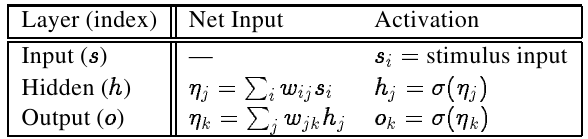
\includegraphics{img/table_bp.png} 
\citet{farkas2013bal} 
\end{center} 


\subsection{Related models}
\label{sec:overview-models}  

In this section we briefly mention models on which our work was based on. Mainly it's the Bidirectional Activation-based Learning algorithm~(\ref{sec:models-bal}) by~\citet{farkas2013bal} and the Generalized recirculation~(\ref{sec:models-generec}) by~\citet{o1996bio}. The other two models are inspiration for the two former ones. Understanding the latter helps understanding the former. We compare these models to our specialized versions in table~\ref{tab:results-cmp-auto4}. 

%\subsubsection{Boltzmann machines}
TODO \cite{ackley1985learning}


To assess the effect of interactivity, two different networks were compared on the combinatorial generaliza-
tion task, a standard feedforward backpropagation network, and an interactive GeneRec network using the
symmetric, midpoint variation learning rule which is equivalent to contrastive Hebbian learning (CHL) or a
deterministic Boltzmann machine (DBM) \cite{o1996bio}, \cite{o2001generalization}. 

TODO: Read and cite from Hinton's original article. 

(Wiki) A Boltzmann machine is a type of stochastic recurrent neural network invented by Geoffrey Hinton and Terry Sejnowski. Boltzmann machines can be seen as the stochastic, generative counterpart of Hopfield nets. They were one of the first examples of a neural network capable of learning internal representations, and are able to represent and (given sufficient time) solve difficult combinatoric problems. If the connectivity is constrained, the learning can be made efficient enough to be useful for practical problems.

A Boltzmann machine, like a Hopfield network, is a network of units with an "energy" defined for the network. It also has binary units, but unlike Hopfield nets, Boltzmann machine units are stochastic. The global energy, $E$, in a Boltzmann machine is identical in form to that of a Hopfield network:

$$E = -\sum_{i<j} w_{ij} \, s_i \, s_j - \sum_i \theta_i \, s_i.$$

Where:
\begin{itemize}
    \item $w_{ij}$ is the connection strength between unit $j$ and unit $i$.
    \item $s_i$ is the state, $s_i \in \{0,1\}$, of unit $i$
    \item $\theta_i$ is the threshold of unit $i$.
\end{itemize}

The connections in a Boltzmann machine have two restrictions:
\begin{itemize}
    \item $w_{ii}=0\qquad \forall i$. (No unit has a connection with itself.)
    \item $w_{ij}=w_{ji}\qquad \forall i,j$. (All connections are symmetric.)
\end{itemize}

Often the weights are represented in matrix form with a symmetric matrix $W$, with zeros along the diagonal.

\paragraph{Hopfield nets.}

TODO: Read and cite from Hopfields's original article. (Storkey, Amos. "Increasing the capacity of a Hopfield network without sacrificing functionality." Artificial Neural Networks—ICANN'97 (1997): 451-456.)

(Wiki) A Hopfield network is a form of recurrent artificial neural network invented by John Hopfield. Hopfield nets serve as content-addressable memory systems with binary threshold nodes. They are guaranteed to converge to a local minimum, but convergence to a false pattern (wrong local minimum) rather than the stored pattern (expected local minimum) can occur. Hopfield networks also provide a model for understanding human memory.

\paragraph{Boltzmann distribution.}

TODO:  Landau, Lev Davidovich; and Lifshitz, Evgeny Mikhailovich (1980) [1976]. Statistical Physics. 5 (3 ed.). Oxford: Pergamon Press. ISBN 0-7506-3372-7. Translated by J.B. Sykes and M.J. Kearsley. See section 28

(Wiki) The Boltzmann distribution for the fractional number of particles $Ni / N$ occupying a set of states $i$ possessing energy $E_i$ is:

    $${N_i \over N} = {g_i e^{-E_i/(k_BT)} \over Z(T)}.$$

where $k_B$ is the Boltzmann constant, $T$ is temperature (assumed to be a well-defined quantity), $g_i$ is the degeneracy (meaning, the number of levels having energy $E_i$; sometimes, the more general \'states\' are used instead of levels, to avoid using degeneracy in the equation), $N$ is the total number of particles and $Z(T)$ is the partition function.

    $$N=\sum_i N_i,$$

    $$Z(T)=\sum_i g_i e^{-E_i/(k_BT)}. $$
  %moved to old 

%\def\myover#1#2{\mathrel{\overset{\makebox[0pt]{#2}}{#1}}}
%\newcommand{\mytilde}{\raise.17ex\hbox{$\scriptstyle\mathtt{\sim}$}}
%\def\myequi#1{\myover{#1}{\mytilde}}

\subsubsection{Contrastive Hebbian learning}
\label{sec:models-chl} 

The main idea of \emph{Contrastive Hebbian Learning} developed by~\citet{movellan1990contrastive} is to have two activation phases in an aribtrary Hopfield network~\citep{hopfield1984neurons} as described in~Section~\ref{sec:theory-hopfield}. In the first phase, called \emph{minus phase} and denoted ``$-$'', only the input vector is \emph{clamped}, i.e. activations of the clamped units as equal to the clamped values. In the second phase, called \emph{plus phase} and denoted ``$+$'', both the input and target are clambed to the underlying network. The learning is based on the difference of these two activations. For an idea how it works see Table~\ref{tab:models-generec}. Note that CHL makes no assumptions about the structure of the underlying network and therefore, it has no layers in general. 

\newpage
As mentioned previously CHL is based on Hopfield networks. Therefore, it has an energy function $J$ which is based on the Helmholtz free energy function $F$~\citep{hinton1989deterministic}:
\begin{equation}
  \label{eq:models-chl-helmholtz}
  F = -\frac{1}{2}\sum_i\sum_ja_iw_{ij}a_j + \sum_i \int_{f(0)}^{a_i} f_i^{-1}(a)da
\end{equation} 
where $-\frac{1}{2}\sum_i\sum_ja_iw_{ij}a_j$ is the Hopfield energy function~(\ref{eq:theory-hopfield-energy}). Then the \emph{contrastive} error function $J$ is defined as: 
\begin{equation}
  \label{eq:models-chl-energy}
  J = \hat{F^{+}} - \hat{F^{-}}
\end{equation} 
where $\hat{F^{+}}$ and $\hat{F^{-}}$ respectively are the values of the energy functions at equilibrium states for the plus and the minus phases. 

Based on the contrastive energy function~(\ref{eq:models-chl-energy}) a~learning rule is derived by~\citet{movellan1990contrastive}: 
\begin{equation}
  \label{eq:models-chl-learning-rule}
  \Delta w_{ij} = \hat{a_i}^{+}\hat{a_j}^{+} - \hat{a_i}^{-}\hat{a_j}^{-}
\end{equation}
where $\hat{a_i}$ and $\hat{a_j}$ denote the equilibrium state activations of the $i$--th and $j$--th unit. It could be shown that the learning rule~(\ref{eq:models-chl-learning-rule}) decreases the energy function~(\ref{eq:models-chl-energy})~\citep{movellan1990contrastive}. Moreover it could be shown that the CHL learning rule is equivalent to backpropagation learning rule in terms of computability while it is biologically more plausible as it uses only activation for computing the error gradient~\citep{o1996bio, xie2003equivalence}. 

   


%\subsubsection{Almeida-Pineda Algorithm}

Pineda first applied the backpropagation rule to recurrent networks. Recurrent networks can have cycles and they contain no layers. Subset $\Omega$ of the units is treated as the output layer. So the Almeida-Pineda network is a generealization of the backpropagation network. 

As the network is recurrent it can remember information and can be used as CAM.
%TODO citation for CAM 

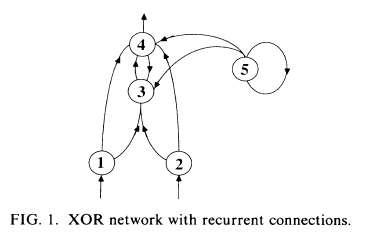
\includegraphics[width=8px]{img/recurrent.png}

\paragraph{My notes.} 
So the Pinedas NS is a dynamical system which should converge and converges for forward/backward nets (quite trivially). 

The delta rule is constructed to move the state towards the fixed point which is defined so that the difference on output neurons is equal to zero (values on other neurons are chosen arbitrary?). 

First Pineda derives an exact learning rule which requires computation of inverse matrix what is both bad for implementation and biological plausibility. So it is simplified to associate dynamical system (I don't understand how) which converges if the original dynamical system converges (proved by Almeida). 

It is more natural as all neurons are equivalent by construction. The advantage is exploited in hardware computation as it treats differential equations more naturally can be solved by analog computers. 

%TODO: Compare this conclusion with O'Reillys. 


TODO: Understand the basics of differential equations to enhance the intuition about learning rules. 

TODO: Study the Lapedes and Farber: master / slave NS. 

\paragraph{Citations from the article.}

Nevertheless it has been applied to recurrent networks by taking advanage of the fact that for every recurrent network there exists an equivalent feedforward network (for a finite time) \cite{pineda1987generalization}.

Hopfield's equations are globally asymptotically stable if $w$ is symmetric and has zeros along the diagonal \cite{pineda1987generalization}.

$$y_r = \beta f_r^,(u_r)\sum_k J_k(L^{-1})_{kr},$$
where 
$$L_{ij} = \alpha \delta_{ij} - \beta f_i^,(u_i)w_{ij},$$
and where $\delta_{ij}$ is the Kronecker $\delta$ symbol and $J_i = t_t - x_i$ if $i \in \Omega$ and $J_i = 0$ otherwise \cite{pineda1987generalization}. 

Then the exact learning rule is 
$$dw_{rs}/dt = \gamma y_r x_s.$$
Rhis exact learning rule needs matrix inversion to calculate the error signals $y_k$. Direct matrix inversions are necessarily nonlocal calculations and therefore this learning algorithm is not suitable for implementation as a neural network \cite{pineda1987generalization}. 

TODO: Understand the associated dynamical system and the new learning rule (page 3/4). 

\paragraph{O'Reillys conclusion}
\cite{o1996bio}
The activation states in AP are updated according to a discrete-time approximation of the following dif-
ferential equation, which is integrated over time with respect to the net input terms :

$$\frac{d\eta_j}{d_t} = -\eta_j + \sum w_{ij} \sigma(\eta_i).$$

This equation can be iteratively applied until the network settles into a stable equilibrium state (i.e., until the
change in activation state goes below a small threshold value), which it will provably do if the weights are
symmetric (Hopfield, 1984), and often even if they are not (Galland \& Hinton, 1991).

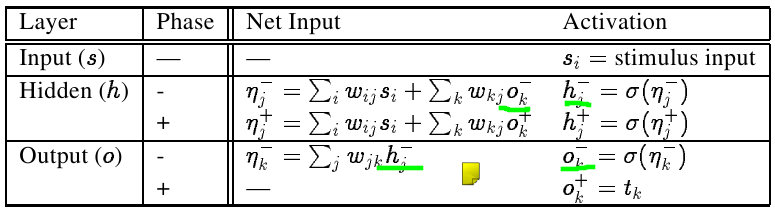
\includegraphics[width=10cm]{img/table_ap.png}
  %moved to old 

\subsubsection{Recirculation algorithm}
\label{sec:models-recirc} 

The \emph{Recirculation algorithm} designed by \citet{hinton1988learning} is an unsupervised neural letwork for learning encoder tasks. Motivation for such a model comes from interesting hidden representations of Backpropagation (\ref{sec:models-bp}) with possible usage as an encoder. It has only two layers denoted \emph{visible layer} and \emph{hidden layer} as shown on figure~\ref{fig:models-recirc}. The aim of the network is to remember on the hidden layer the patterns presented to the visible layer. This could be used for compression if the hidden layer has less units than the visible layer. It also could be used as a content--accessed--memory where if novel patterns are presented to the network it could show the most similar stored pattern. 

\begin{figure}[H]
  \centering
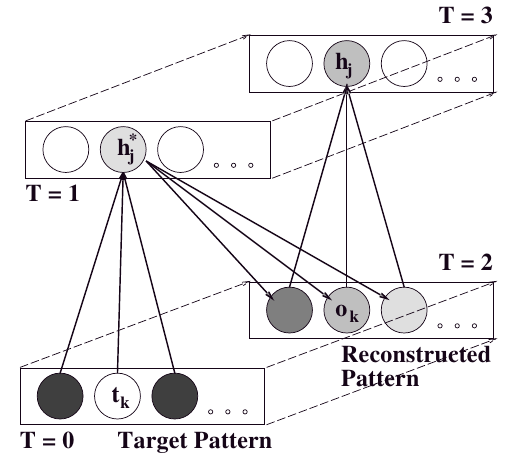
\includegraphics[width=0.4\textwidth]{img/recirculation.png}
  \caption{The recirculation algorithm by \citet{hinton1988learning}. }
  \label{fig:models-recirc}
\end{figure}

As depicted on \ref{fig:models-recirc} activation is propagated in four steps $T \in \{0,1,2,3\}$. At the first phase denoted by $T=0$ only the input vector $t$ is clamped on the visible layer, at $T=1$ a forward pass $h^{*}$ is computed from visible to hidden, at $T=2$ a reconstructed pattern $o_k$ as a function of hidden state $h^{*}$ at $T=1$ is computed and finally at $T=3$ a hidden state $h$ is computed from $o_k$.

For the reconstruction to work \emph{symmetric} weights are used. The learning rule is common for both visible and hidden layers and it;s based only on difference of activations: 
\begin{align}
\frac{\partial E}{\partial w_{ij}} &= -(\eta^{*}_j - \eta_j) \phi'(\eta_j) t_k \nonumber \\
&\approx -(h^{*}_j - h_j)t_k \nonumber 
\end{align} 
The approximation step could be made because $\phi'(\eta_j)$ has \emph{usually} same sign as $(\eta^{*}_j - \eta_j) $ \citep{hinton1988learning, o1996bio}. The approximation works better if the difference of activations is smaller and therefore the activation for the reconstructed pattern $o$  is made similar to target pattern $t$: 
\begin{equation}
o_k = \alpha t_k + (1-\alpha)f(\eta_k). 
\end{equation} 

%Authors study the case of asymetric weights. They do not provide a proof of convergence but they provide some intutition why it should work. Also they link the work of Ballard who experimented with connecting (merging) several closed loops so that hidden units of closed loops can be input units of other closed loops of recirculation.

%\paragraph{From the original article.}
%Instead of using a separate group of units for the input and output we use the very same group of \textit{visible} units, so the input vector is the initial state of this group and the output vector is the state after information has passed around the loop. The difference between the activity of a visible unit before and after sending activity around the loop is the derivative of the squared reconstruction error \citet{hinton1988learning}.

%On the first pass, the original visible vector is passed around the loop, and on the second pass ana average of the original vector and the reconstructed vector is passed around the loop. The learning procedure changes each weight by an amount proportional to the product of the \textit{presynaptic} activity and the \textit{difference} in the post-synaptic activity on the two passes  \citet{hinton1988learning}.



%\subsubsection{Deep architectures}
Theoretical results strongly suggest that in order to learn the kind of complicated functions that can represent high-level abstractions (e.g. in vision, language, and other AI-level tasks), one needs deep architectures. Deep architectures are composed of multiple levels of non-linear operations, such as in neural nets with many hidden layers or in complicated propositional formulae re-using many sub-formulae. Searching the parameter space of deep architectures is a difficult optimization task, but learning algorithms such as those for Deep Belief Networks have recently been proposed to tackle this problem with notable success, beating the state-of-the-art in certain areas. This paper discusses the motivations and principles regarding learning algorithms for deep architectures, in particular those exploiting as building blocks unsupervised learning of single-layer models such as Restricted Boltzmann Machines, used to construct deeper models such as Deep Belief Networks \cite{bengio2009learning} (Abstract copied).

TODO read the article. 
 %moved to old 

\subsubsection{Generalized recirculation}
\label{sec:models-generec} 

\paragraph{Introduction.} 
The \emph{Generalized recirculation algorithm}, or \emph{GeneRec}, was developed by \citet{o1996bio}. It's a supervised algorithm which in comparison with Backpropagation (\ref{sec:models-bp}) is argued to be a more biologically plausible model as error is computed locally as a difference between activations \citep{o1998six, o2001generalization, da2011advances, schneider2009application}. In summary, GeneRec is a combination of CHL (\ref{sec:models-chl}) and the Recirculation algorithm (\ref{sec:models-recirc}). It overcomes limitations of the Recirculation algorithm to be an encoder by having a three layer network. For the error computation a backward weight matrix from output layer to hidden layer is used and the learning rule is derived from the CHL learning rule~\ref{eq:models-chl-learning-rule}. It could be proven that GeneRec, as Backpropagation, could learn arbitrary input--output mappings \citep{o1996bio}. 

\paragraph{Learning rule.} 
\label{sec:models-generec-learning-rule} 
GeneRec uses three weight matrices $W^{IH}$, $W^{HO}$ and $W^{OH}$ for the input--hidden, hidden--output and output--hidden weights. It also has the \quotes{-} and \quotes{+} phases as CHL with same meaning, i.e. in the \emph{minus} phase only the input vector is clamped and in the \emph{plus} phase both input and target vectors are clamped as seen on table~\ref{tab:models-generec}. Generec uses the non--symmetric version of the CHL rule for all three weight matrices: 
\begin{equation}
  \label{eq:models-generec-learning-rule}
  \Delta w_{ij} = \lambda a^{-}_i(a^{+}_j - a^{-}_j)
\end{equation}
where $a^{-}_p$ denotes the presynaptic and $a^{-}_q$ denotes the postsynaptic unit activation in minus phase, $a^{+}_p$ is the presynaptic activation from plus phase and $\lambda$ denotes the learning rate. So for example when updating $W^{HI}$ then $a^{-}_i = h^{-}_i$, $a^{-}_j = o^{-}_j$ and $a^{+}_j = t_k$. 

\paragraph{Activation.} 
\label{sec:models-generec-activation} 
The main difference between CHL and GeneRec is that GeneRec has layers and it's based more on Recurrent neural networks than on the Hopfield networks. Therefore, as shown in table~\ref{tab:models-generec}, we can compute the activations sequentially. 
\begin{table}[H]
  \centering
  \begin{tabular}{|cccc|}
    \hline
    Layer & Phase & Net Input & Activation\\
    \hline
    Input (s)    & $-$ & - & $s_i$ = \mbox{stimulus input} \\
    \hline
    Hidden (h)   & $-$ & \hspace{0.3cm}$\eta^{-}_j = \sum_i w_{ij}^{IH}s_i + \sum_k w_{kj}^{OH}o^{-}_k$\hspace{0.3cm} &
    $h^{-}_j = \sigma(\eta^{-}_j)$\hspace{0.3cm}\\
          &  +  & $\eta^{+}_j = \sum_{i}w_{ij}^{IH}s_i + \sum_k w_{kj}^{OH}o^{+}_k$ & $h^{+}_{j} = \sigma(\eta^{+}_j)$ \\
    \hline
    Output (o) & $-$ & $\eta^{-}_k = \sum_j w_{jk}^{HO}h_j$ & $o^{-}_k = \sigma(\eta^{-}_k)$\\
           &  +  & - & $o^{+}_k$ = \mbox{target output} \\
    \hline
  \end{tabular}
  \caption{Equilibrium network variables in GeneRec model \citet{o1996bio}. We can see the inspiration from the Recirculation algorithm (\ref{sec:models-recirc}) and a correspondence between $T$ and GeneRec phases. In particular $s^{-} \approx T=0$, $h^{-} \approx T=1$, $o^{-} \approx T=2$ and $h^{+}$ corresponds to $T=3$. The activation flow is depicted on figure~\ref{fig:models-generec-phase}.}
  \label{tab:models-generec}
\end{table}
In case of the \emph{plus} phase only the hidden activations are necessary to compute what could be achieved by computing $\phi(\eta_i)$. In case of the \emph{minus} phase where only inputs are clamped it's necessary to find an \emph{equilibrium} activation state for which the equations~\ref{tab:models-generec} hold. As dicussed in recurrent networks~(\ref{sec:theory-recurrent}) there are several approaches. In our implementation~(\ref{sec:appendix-impl-generec}) we choose the \emph{iterative method} with following rules for computing activations $a_i$: 
\begin{align}
  \label{eq:models-generec-activation}
  a_i(0) &= \left\{
	\begin{array}{ll}
		s_i & \mbox{if } i \in \mbox{input} \nonumber \\
		0 & \mbox{otherwise} \nonumber 
	\end{array}
\right. \\
  a_i(t+1) &= \left\{
	\begin{array}{ll}
		s_i & \mbox{if } i \in \mbox{input} \nonumber \\
		\phi(\sum_j w_{ji}a_j(t)) & \mbox{otherwise} \nonumber 
	\end{array}
\right. \\
\end{align} 
where $a_i(t)$ is the activation of $i$--th unit in discrete time $t$. The rules~\ref{eq:models-generec-activation} while are iterated while $|a_i(t+1) a_i(t)| > \epsilon$ for some unit $i$. This method is further discussed in (\ref{sec:generec-fluctuation}) and \citep{orru2008sabio}.

\begin{figure}[H]
  \centering
  %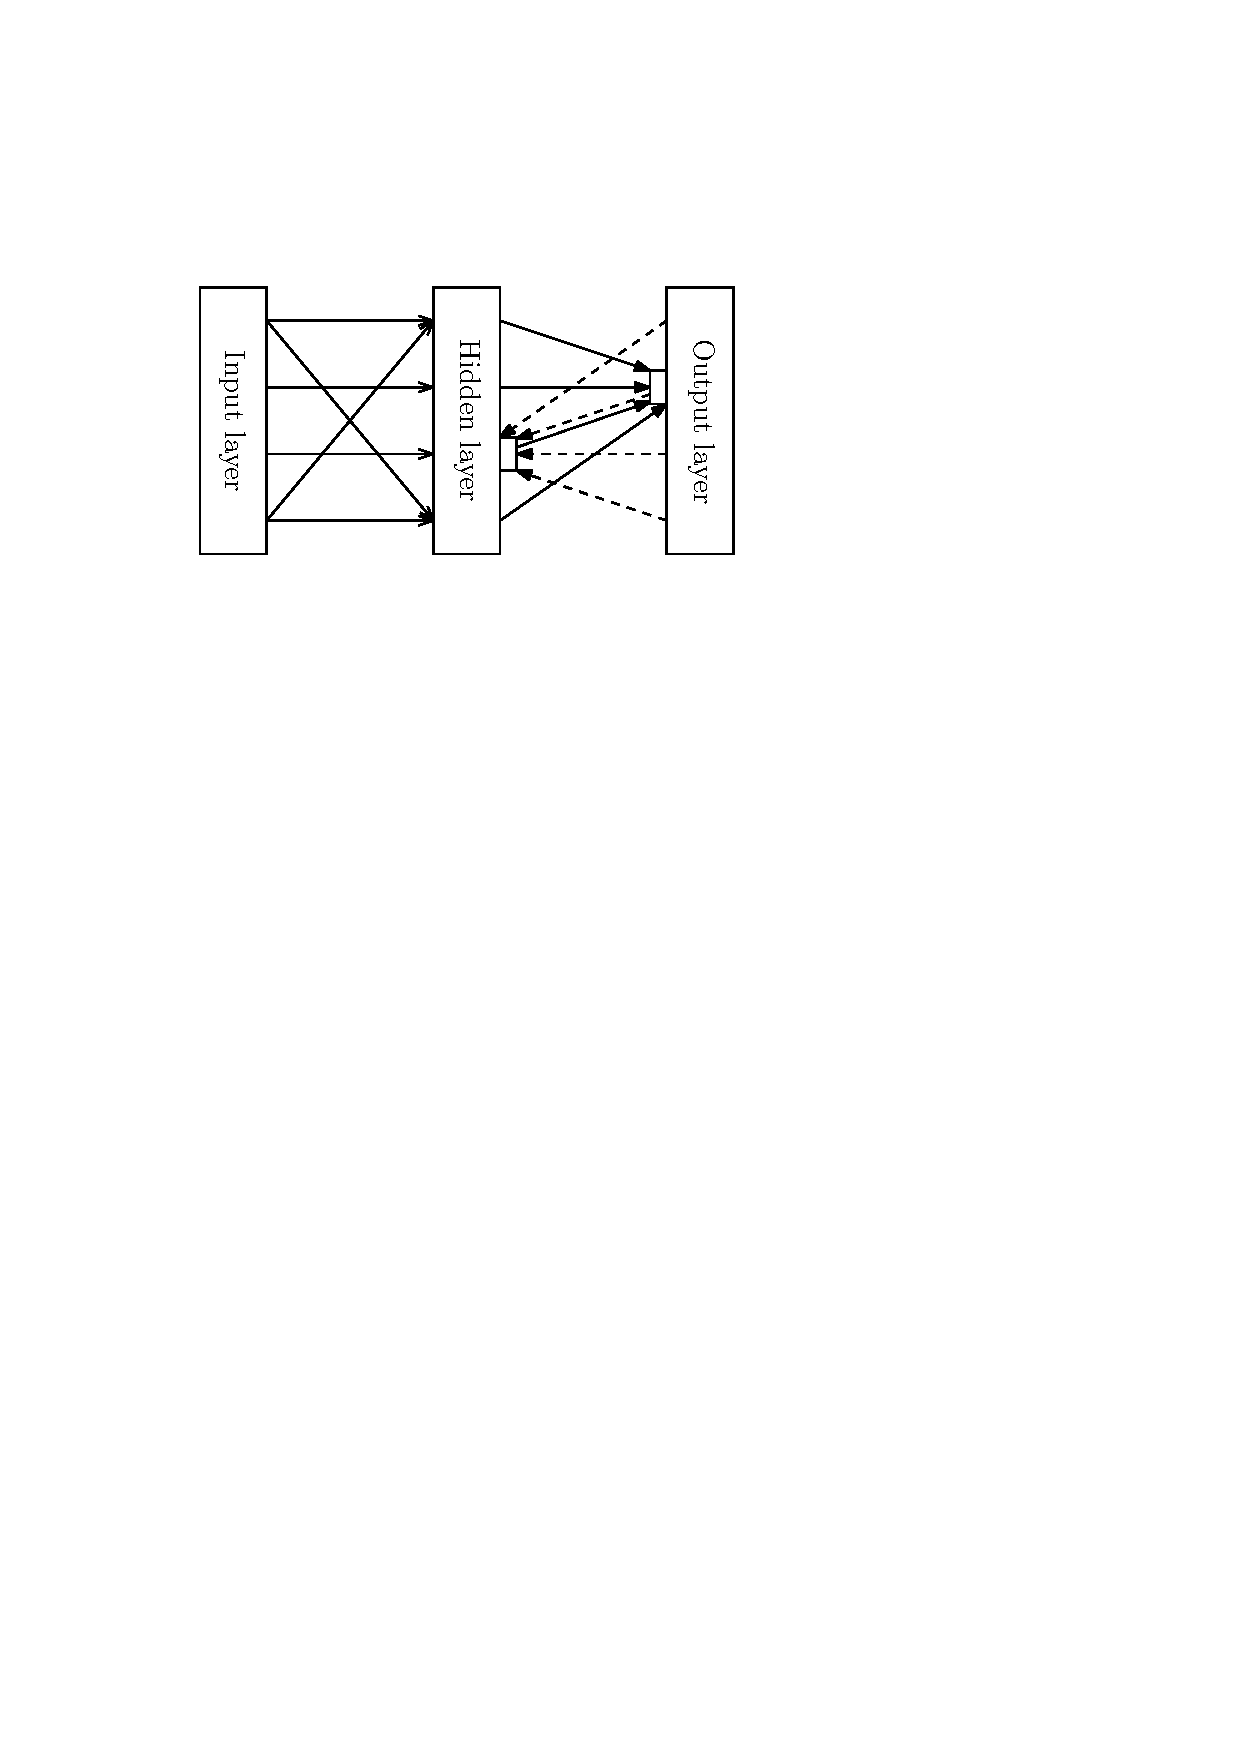
\includegraphics[width=0.4\textwidth,left]{img/models-generec-minus-phase.pdf}
  %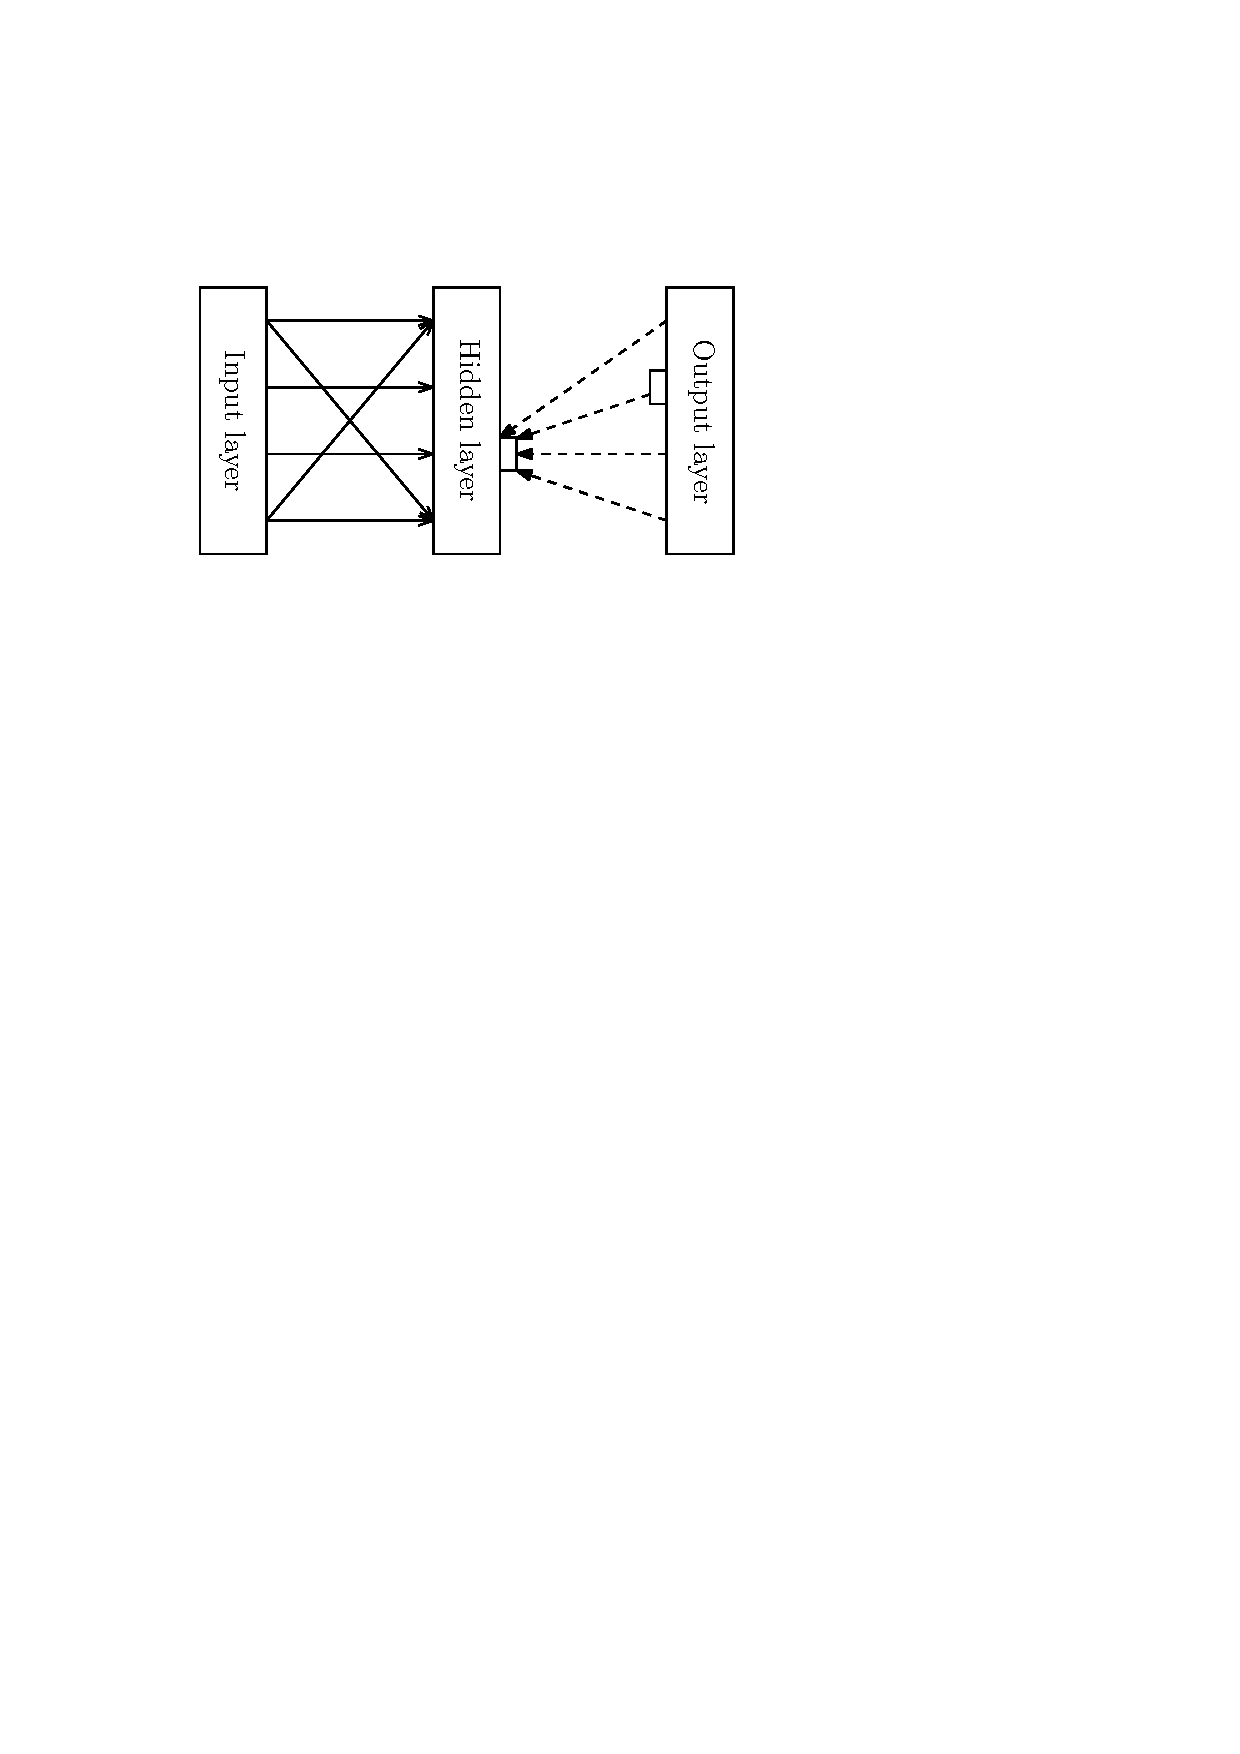
\includegraphics[width=0.4\textwidth,right]{img/models-generec-plus-phase.pdf}
  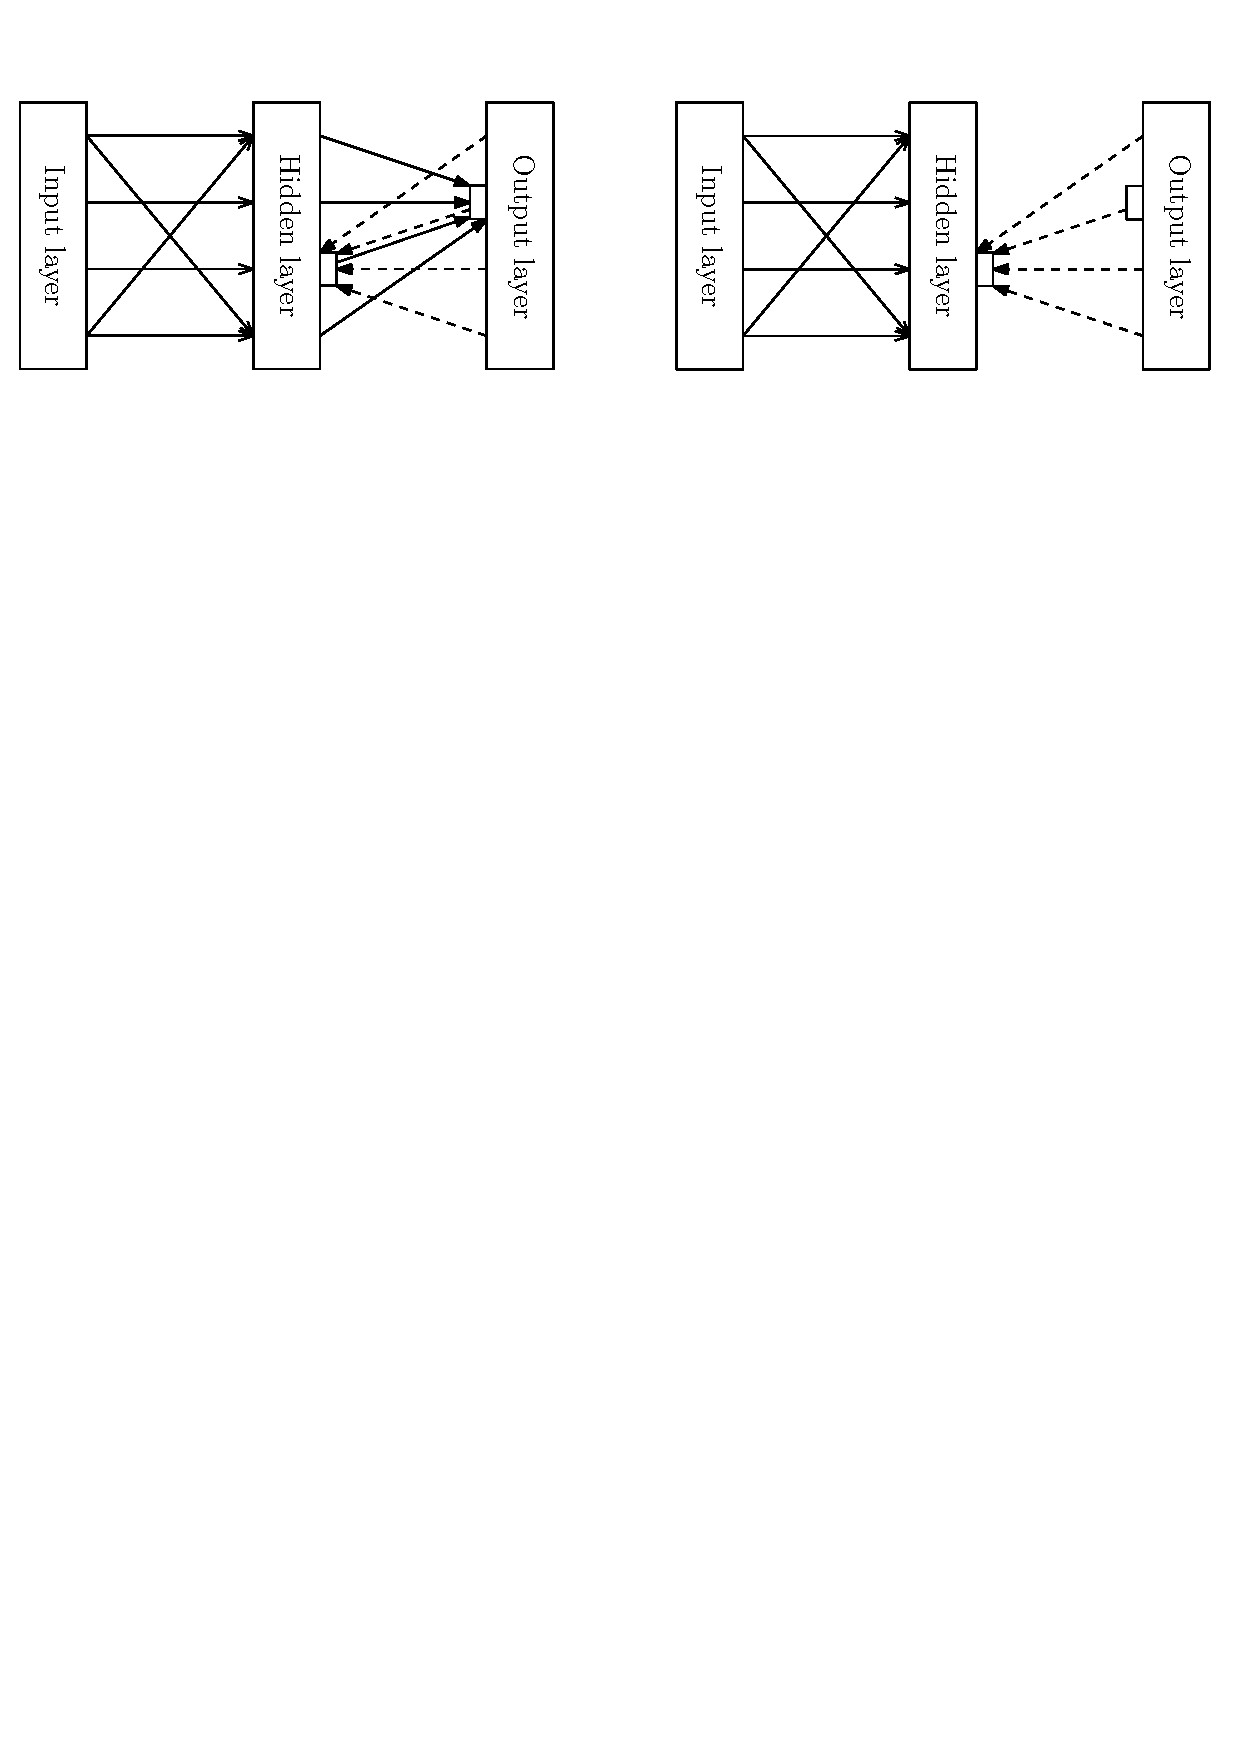
\includegraphics[width=0.8\textwidth]{img/models-generec-phase.pdf}
  
  \caption{Depicting the minus (left) and plus (right) phases of GeneRec defined in table~\ref{tab:models-generec}. Picture inspiration from \citet{orru2008sabio}.} 
  \label{fig:models-generec-phase}
\end{figure}

\paragraph{Modifications.}
\label{sec:our-learning-rules}
\label{sec:models-generec-modifications} 
It's important to note that \citet{o1996bio} proved that GeneRec converges if the learning rule~\ref{eq:models-generec-learning-rule} is a valid approximation to the error derivate and the weights beeing symmetric, i.e. $W^{HO} = W^{OH^{T}}$. \citet{o1996bio} based on CHL and the midpoint method for fradient computation \citep{press1990numerical} proposed two more learning rules for GeneRec: 
\begin{equation}
  \label{eq:models-generec-learning-rule-mid}
  \frac{1}{\lambda} \Delta w_{ij} =  \frac{1}{2}(a^{-}_i + a^{+}_i)(a^{+}_j - a^{-}_j)
\end{equation}
\begin{equation}
  \label{eq:models-generec-learning-rule-sym}
  \frac{1}{\lambda} \Delta w_{ij} =  (a^{+}_j a^{-}_i - a^{-}_j a^{+}_i) - 2a^{-}_j a^{-}_i
\end{equation}
where~\ref{eq:models-generec-learning-rule-mid} is called the \emph{midpoint learning rule} and~\ref{eq:models-generec-learning-rule-sym} is called the \emph{symmetric learning rule} which aims to preserve weight symmetry. By combining rules ref{eq:models-generec-learning-rule-mid} and \ref{eq:models-generec-learning-rule-sym} we get the following rule: 
\begin{equation}
  \label{eq:models-generec-learning-rule-chl}
  \frac{1}{\lambda} \Delta w_{ij} =  (a^{+}_i a^{+}_j) - (a^{-}_i a^{-}_j)
\end{equation}
which is indeed the CHL learning rule~\ref{eq:models-chl-learning-rule}. Thus we see that GeneRec is closely related to CHL. 

Note that we encountered some missing details in \citet{o1996bio} about how to implement the GeneRec algorithm which are further discussed in (\ref{sec:appendix-impl-generec}).


%==================== 12.   Background overview (optional) ======
\subsection{Bidirectional Activation-based Learning algorithm} 
\label{sec:models-bal} 
% If your work builds on top of an existing one, this is the place to describe the existing work in more detail, pointing out the parts that you extend or improve and why you extend or improve these parts.

Design of Bidirectional Activation-based Learning algorithm (BAL) by \citet{farkas2013bal} is motivated by the biological plausibility of GeneRec. BAL inherits the learning rule of GeneRec \ref{eq:models-generec-learning-rule} and also the two phases. But unlike GeneRec, BAL aims to learn bidirectional mapping between inputs and outputs and for this purpose it uses four weights $W^{IH}$, $W^{HO}$, $W^{OH}$ and $W^{HI}$. The design of BAL is symmetric as shown in table~\ref{tab:models-bal-activation} and thus we avoid calling inputs, outpus, minus phase or plus phase. We rather choose \emph{forward} and \emph{backward} which could be interchanged. Note that the forward activations are denoted as $a^{\rm F}$ and backward activations as $a^{\rm B}$. 

\begin{table}[H]
  \centering
  \begin{tabular}{|cccl|}
    \hline
    Layer & Phase & Net Input & Activation\\
    \hline
    \Bx & F & - & $x^{\rm F}_i$ = stimulus\\ [1ex]
    \Bh & F & \hspace{0.3cm}$\eta^{\rm F}_j = \sum_i w_{ij}^{IH}x^{F}_i$\hspace{0.3cm} & $h^{\rm F}_j = \sigma(\eta^{\rm F}_j)$\hspace{0.3cm}\\ [1ex]
    \By & F & $\eta^{\rm F}_k = \sum_j w_{jk}^{HO}h^{F}_j$ & $y^{\rm F}_k = \sigma(\eta^{\rm F}_k)$\\ [1ex]
    \hline
    \By & B & - & $y^{\rm B}_k$ = stimulus\\ [1ex]
    \Bh & B & $\eta^{\rm B}_j = \sum_k w_{kj}^{OH}y^{\rm B}_k$ & $h^{\rm B}_j = \sigma(\eta^{\rm B}_j)$\\ [1ex]
    \Bx & B  & $\eta^{\rm B}_i = \sum_j w_{ji}^{HI}h^{\rm B}_j$ & $x^{\rm B}_i = \sigma(\eta^{\rm B}_i)$\\
    \hline
  \end{tabular}
  \caption{Activation phases and states in BAL \citep{farkas2013bal}. Where \Bx is the first activation layer, i.e. \emph{front layer}, \By is the third activation layer, i.e. \emph{back layer}, $F$ means \emph{forward pass} and $B$ means \emph{backward pass}. Layers \Bx and \By are \emph{visible} and layer \By is hidden. Note that all non--stimulus units have learnable biases and their weights are updated in a same way as regular weights.} 
  \label{tab:models-bal-activation}
\end{table}

In the first phase called \emph{forward pass} the \emph{forward stimulus} is clamped and forward activations are computed. In the same way, in the second phase called \emph{backward pass} the \emph{backward stimulus} is clamped and backward activations are computed. We can imagine the backward pass as a reconstruction of the target pattern for the forward pass. For the learning rule the \emph{difference} between the forward pass and the backward pass is used: 
\begin{equation}
  \label{eq:models-bal-learning-rule-forward}
  \Delta w_{ij}^{\rm F} = \lambda \ a_i^{\rm F}(a_j^{\rm B} - a_j^{\rm F}),
\end{equation}
and for completeness we also provide the backward learning rule which is same as the forward learning rule~\ref{eq:models-bal-learning-rule-forward}: 
\begin{equation}
  \label{eq:models-bal-learning-rule-backward}
  \Delta w_{ij}^{\rm B} = \lambda \ a_i^{\rm B}(a_j^{\rm F} - a_j^{\rm B}). 
\end{equation}
Note that we can treat the differences $(a_j^{\rm B} - a_j^{\rm F})$ and $(a_j^{\rm F} - a_j^{\rm B})$ as \emph{error terms} which push the forward and backward activation to settle. Both forward~\ref{eq:models-bal-learning-rule-forward} and backward~\ref{eq:models-bal-learning-rule-backward} learning rules are same as the basic GeneRec learning rule~\ref{eq:models-generec-learning-rule}. We experimented with different learning rules (\ref{sec:our-learning-rules}). 

 


 
